\chapter{Einf\"urung}
\label{chap:introduction}
Tagt{\"a}glich tauschen Millionen von Nutzern {\"u}ber Social Media Informationen zu verschiedenen Themen aus. Eine der bekanntesten Plattformen ist Twitter: eine Microblogging-Plattform, die sich grosser Beliebtheit erfreut und weltweit eingesetzt wird. Microblogging ist eine spezielle Form des Bloggens und unterscheidet sich vom klassischen Blogging vor allem durch die L{\"a}nge der Eintr{\"a}ge. Seit November 2017 betr{\"a}gt die maximale L{\"a}nge der Nachrichten auf Twitter 280 Unicode-Zeichen. Standardm{\"a}ssig ist ein Beitrag, ein sogenannter ``Tweet'', {\"o}ffentlich und auch f{\"u}r nicht registrierte Benutzer sichtbar. Die Tweets werden haupts{\"a}chlich den Followern angezeigt, aber {\"u}ber Hashtags und/oder Links oder Retweets kann eine breite Masse auf der ganzen Welt erreicht werden.

Leider haben Hasskommentare, Trolling und Social Media Mobbing in den letzten Jahren zugenommen und sind zu einem ernsthaften Problem geworden. Daf{\"u}r gibt es unterschiedliche Gr{\"u}nde, die zu diesem Anstieg f{\"u}hren: Ein Grund ist sicher die Anonymit{\"a}t des Internets, denn es ist leichter einen abf{\"a}lligen Kommentar zu schreiben, als ihn der betreffenden Person direkt ins Gesicht zu sagen. Doch dies ist nicht die einzige Erkl{\"a}rung. Generell ist zu beobachten, dass sich vermehrt Prominente wie Donald Trump, Jens Maier und Thomas Seitz - letztere beide aus der AfD - oder Josh Hader (Baseballspieler), um nur einige wenige zu nennen, rassistisch in Social Media Kan{\"a}len {\"a}ussern. Durch diesen t{\"a}glichen Gebrauch und der Verbreitung von Hasskommentaren durch Prominente scheint die {\"o}ffentliche Diskreditierung in der Gesellschaft f{\"u}r viele akzeptabel geworden zu sein. 

Doch was genau sind Hasskomentare? Eine Definition: 
\begin{description}
\item[hate speech] speech that attacks, threatens, or insults a person or group on the basis of national origin, ethnicity, color, religion, gender, gender identity, sexual orientation, or disability.  \url{https://www.dictionary.com/browse/hate-speech}
\end{description}

Beispiele f{\"u}r rassistische oder sexistische Tweets:
\begin{itemize}
  \item $@$thumpmomma: I likewise saw militant Muslims burning our flag and burning George Bush photos and figures, right after 9/11! Not\#here!
  \item $@$femfreq the main reason why all the harass to women is because of all the dumb feminist bitches who want to be superior. Hope u die raped
  \item Sir\_Penaut 1.You din't go to colleg. 2. You are black.
  \item You're studying Computer Science? Do you wanna meet boys there and change university when you tried them all?" \#EverydaySexism
  \item Experience Charlie. Married woman who loves hot phone sex with strangers. Can you get me off? - 27 http://t.co/bpDqqPoGAe
\end{itemize}
                                                                                                                                                                                                                                                                                                                                                                                                                                                                                                                                                                                                                                                                                                                                                                                                                                                                                                                                                                                                                                                                                                                                                                                                                                                                                                                                                                                                                                                                                                                                                                                                                                                                                                                                                                                                                                                                                                                                                                       
Die oben aufgef{\"u}hrten Tweets sind in Englisch, da die Modelle (siehe Kapitel \ref{sec:introduction_purpose}) mit englischen Trainingsdaten trainiert wurden und die App nur englischen Text klassifizieren kann.                                                                                                                                                                                                                                                                                                                                                                                                                                                                                                                                                                                                                                                                                                                                                                                                                                                                                                                                                                                                                                                                                                                                                                                                                                                                                                                                                                                                                                                                                                                                                                                                                                                                                                                                                                                                                                                                                                                                                                                                                                                                                                                                                                                                                                                                                                                                                                                                                                                                                                                                                                                                                                                                                                                                                                                                                                                                                                                                                                                                                                                                                                                                                                                                                                                                                                                                                                                                                                                                                                                                                                                                                                                                                                                                                                                                                                                                                                                                                                                                                                               

\begin{figure}[H]
	\centering
		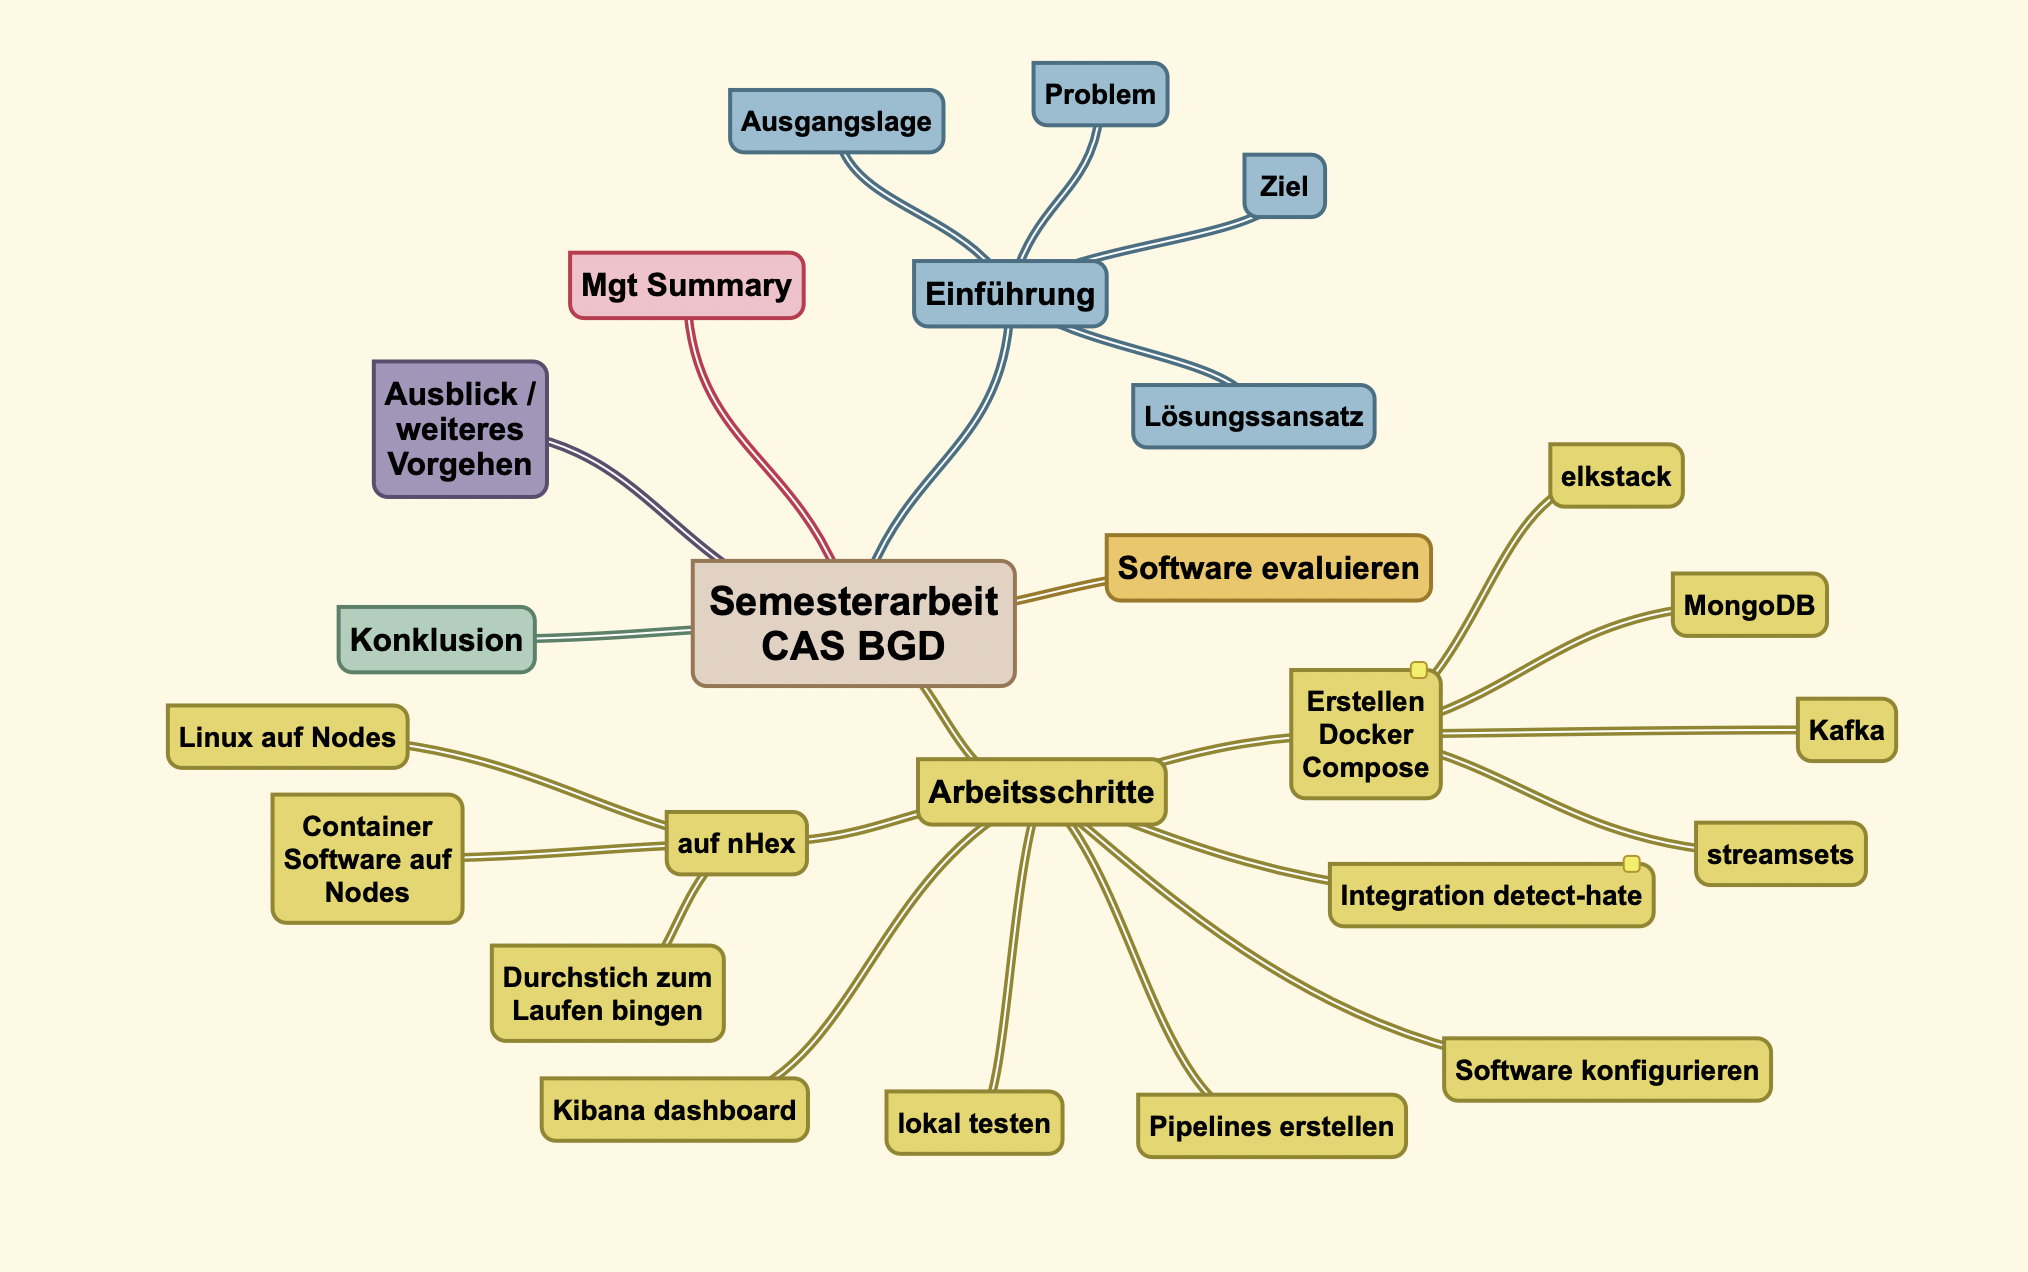
\includegraphics[scale=0.4 ]{images/inhalt_arbeit.png}
	\caption{Inhalt Semsterarbeit}
	\label{fig:inhalt_semesterarbeit}
\end{figure}

Das Vorgehen und der Aufbau dieser Semesterarbeit ist auf Bild \ref{fig:inhalt_semesterarbeit} dargestellt und diese Dokumentation orientiert sich an der Struktur. 

                                                                                                                                                                                                                                                                                                                                                                                                                                                                                                                                                                                                                                                                                                                                                                                                                                                                                                                                                                                                                                                                                                                                                                                                                                                                                                                                                                                                                                                                                                                                                                                                                                                                                                                                                                                                                                                                                                                                                                                                                                                                                                                                                                                                                                                                                                                                                                                                                                                                                                                                                                                                                                                                                                                                                                                                                                                                                                                                                                                                                                                                                                                                                                                                                                                                                                                                                                                                                                                                                                                                                                                                                                                                                                                                                                                                                              \section{Ausgangslage}
\label{sec:introduction_purpose}

Im CAS Practical Machine Learning wurde eine \href{http://www.detect-hate.com}{Flask App} entwickelt um Hasskommentare (hate speech) in Tweets zu erkennen. F{\"u}r die Klassifikation wurden folgende Algorithmen
\begin{itemize}
\item Lineare Support Vector Macine (SVM)
\item Logistic Regression
\item Multinominal Naive Bayes
\item Long short-term memory (LSTM) neuronales Netz
\end{itemize}
verwendet und 20 Modelle trainiert. Als Datengrundlage f{\"u}r die Modelle dienten vier unterschiedliche Datens{\"a}tze aus verschiedenen Quellen mit total ca. 85.000 Tweets. Diese Datens{\"a}tze enthielten nebst den eigentlichen Tweets weitere Spalten, so z.B. die folgenden Labels:
\begin{itemize}
  \item None
  \item Abusive
  \item Sexist
  \item Racist
\end{itemize}
Basierend auf den verwendeten Datens{\"a}tzen und deren Labels wurden die oben genannten Klassifikationsalgorithmen und das Neuronales Netz trainiert, um auch neuen, den Klassifikationen unbekannte Hasskommentare automatisiert zu erkennen. 

\section{Problemstellung }
\label{sec:introduction_	purpose}
Es ist nicht m{\"o}glich die Tweets mit der App automatisch zu klassifizieren. Um zu pr{\"u}fen ob ein Text Hasskommentare enth{\"a}t ist ein manueller Zwischenschritt n{\"o}tig, bei welchem die Tweets von Twitter kopiert und auf der Homepage (www.detect-hate.com) in das Textfeld eingef{\"u}gt wird. Das Resultat, also die Klassifikation ob der Tweet Hasskommentare enth{\"a}lt oder nicht und die dazugeh{\"o}rigen Wahrscheinlichkeiten werden angezeigt, aber nicht gespeichert. Somit ist es nicht m{\"o}glich die Resultate zu analysieren und einen {\"U}berlick {\"u}ber die H{\"a}ufigkeit und Verwendung von Hasskommentaren bei Twitter zu bekommen.

Des Weiteren haben Tests mit neuen, in der Applikation eingegebenen Texten von Twitter (oder auch frei erfunden) gezeigt, dass die trainierten Algorithmen nur bedingt korrekte Aussagen treffen k{\"o}nnen. Dieses Problem liegt insbesondere in den f{\"u}r das Training verwendeten Datens{\"a}tzen:
Zu wenig Trainingsdaten f{\"u}r eine Textklassifikation von Freitext, insbesondere f{\"u}r das Neuronale Netz. Die Tweets der Trainingsdaten wurden jeweils nur {\"u}ber einen sehr kurzen Zeitraum gesammelt, das f{\"u}hrt zu einem grossen Bias Problem (zu dem Erfassungszeitraum behandelte Themen entsprechen nur z.T. den Themen {\"u}ber einen l{\"a}ngeren Zeitraum resp. zur aktuellen Zeit)
Nicht alle Datens{\"a}tze hatten Labels f{\"u}r alle Kategorien von Hasskommentaren (weniger als 10.000 sexistisch und/oder rassistisch gelabelte Daten).

\section{Ziel}
\label{sec:ziel}
Ziel dieser Semesterarbeit ist es eine Streaming und Analyse Umgebung aufzubauen um die Tweets direkt zu klassifizieren und die Resulatete zu speichern. Die daf{\"u}r n{\"o}tigen Schritte beziehungsweise zu erreichende Meilensteine sind folgende:
\begin{itemize}
\item Abgesetzte Tweets von der Twitter API beziehen
\item Unbearbeitet Tweets und Metainformationen in eine Datenbank persistenten um f{\"u}r die Matserarbeit Trainingsdaten zur Verf{\"u}gung zu haben. Mit diesen Daten sollen sp{\"u}ter die Machine Leaerning Modell von  \href{http://www.detect-hate.com} trainiert werden.  
\item Datenaufbereitung der von Twitter bezogenen Daten
\item Hasskommentare in Tweets erkennen, mittels der detect-hate App
\item Tweets und Prognose der Modelle persitieren
\item Dashboard mit den Resultaten erstellen
\end{itemize}

\section{L{\"o}sungsansatz}
\label{sec:introduction_solution}
Da 5.787 Tweets pro Sekunde ver{\"o}ffentlicht werden, soll einen Stream realisiert werden, welche die Daten liest, aufbereitet, verteilt und persistiert. Die eingesetzten Komponenten m{\"u}ssen in der Lage sein, mit dieser grossen Datenmenge in der kurzen Zeit umzugehen. Da die L{\"o}sung zuerst lokal einwickelt wird und sp{\"a}ter ohne grossen Aufwand auf einer Big Data Plattform betrieben werden soll, werden Container genutzt. In \ref{fig:high_level_architecure} ist die Highlevel L{\"o}sungsarchitektur ersichtlich. 

Wie in auf dem Bild \ref{fig:high_level_architecure} Highlevel L{\"o}sungsarchitektur ersichtlich soll eine containernbasierte Lösung realisiert werden, welche die Datensammlung, Aufbereitung, Klassifikation und Speicherung mittels Pipelines umsetzt. Idealerweise wird eine Streaming-Software (ETL) verwendet, welche ein Monitoring und ein hohen Automatisationsgrad bietet um möglichst viele Datenaufbereitungsschritte durchführen zu können. Da 5.787 Tweets pro Sekunde ver{\"o}ffentlicht werden, müssen die eingesetzten  Komponenten in der Lage sein, mit dieser grossen Datenmenge in der kurzen Zeit umzugehen und es muss  genügend Speicher zur Verfügung stehen um die Daten von Twitter und die Resultate zu speichern. Die L{\"o}sung wird zuerst lokal einwickelt und sp{\"a}ter ohne grossen Aufwand auf einer Big Data Plattform portiert. Die favorisierte Big Data Plattform ist on-prem, der BigBoards Cluster "nHex i3", welcher in meinem Keller steht. Alternativ kommt ein Cloud Ansatz in Frage. 

\begin{figure}[H]
	\centering
		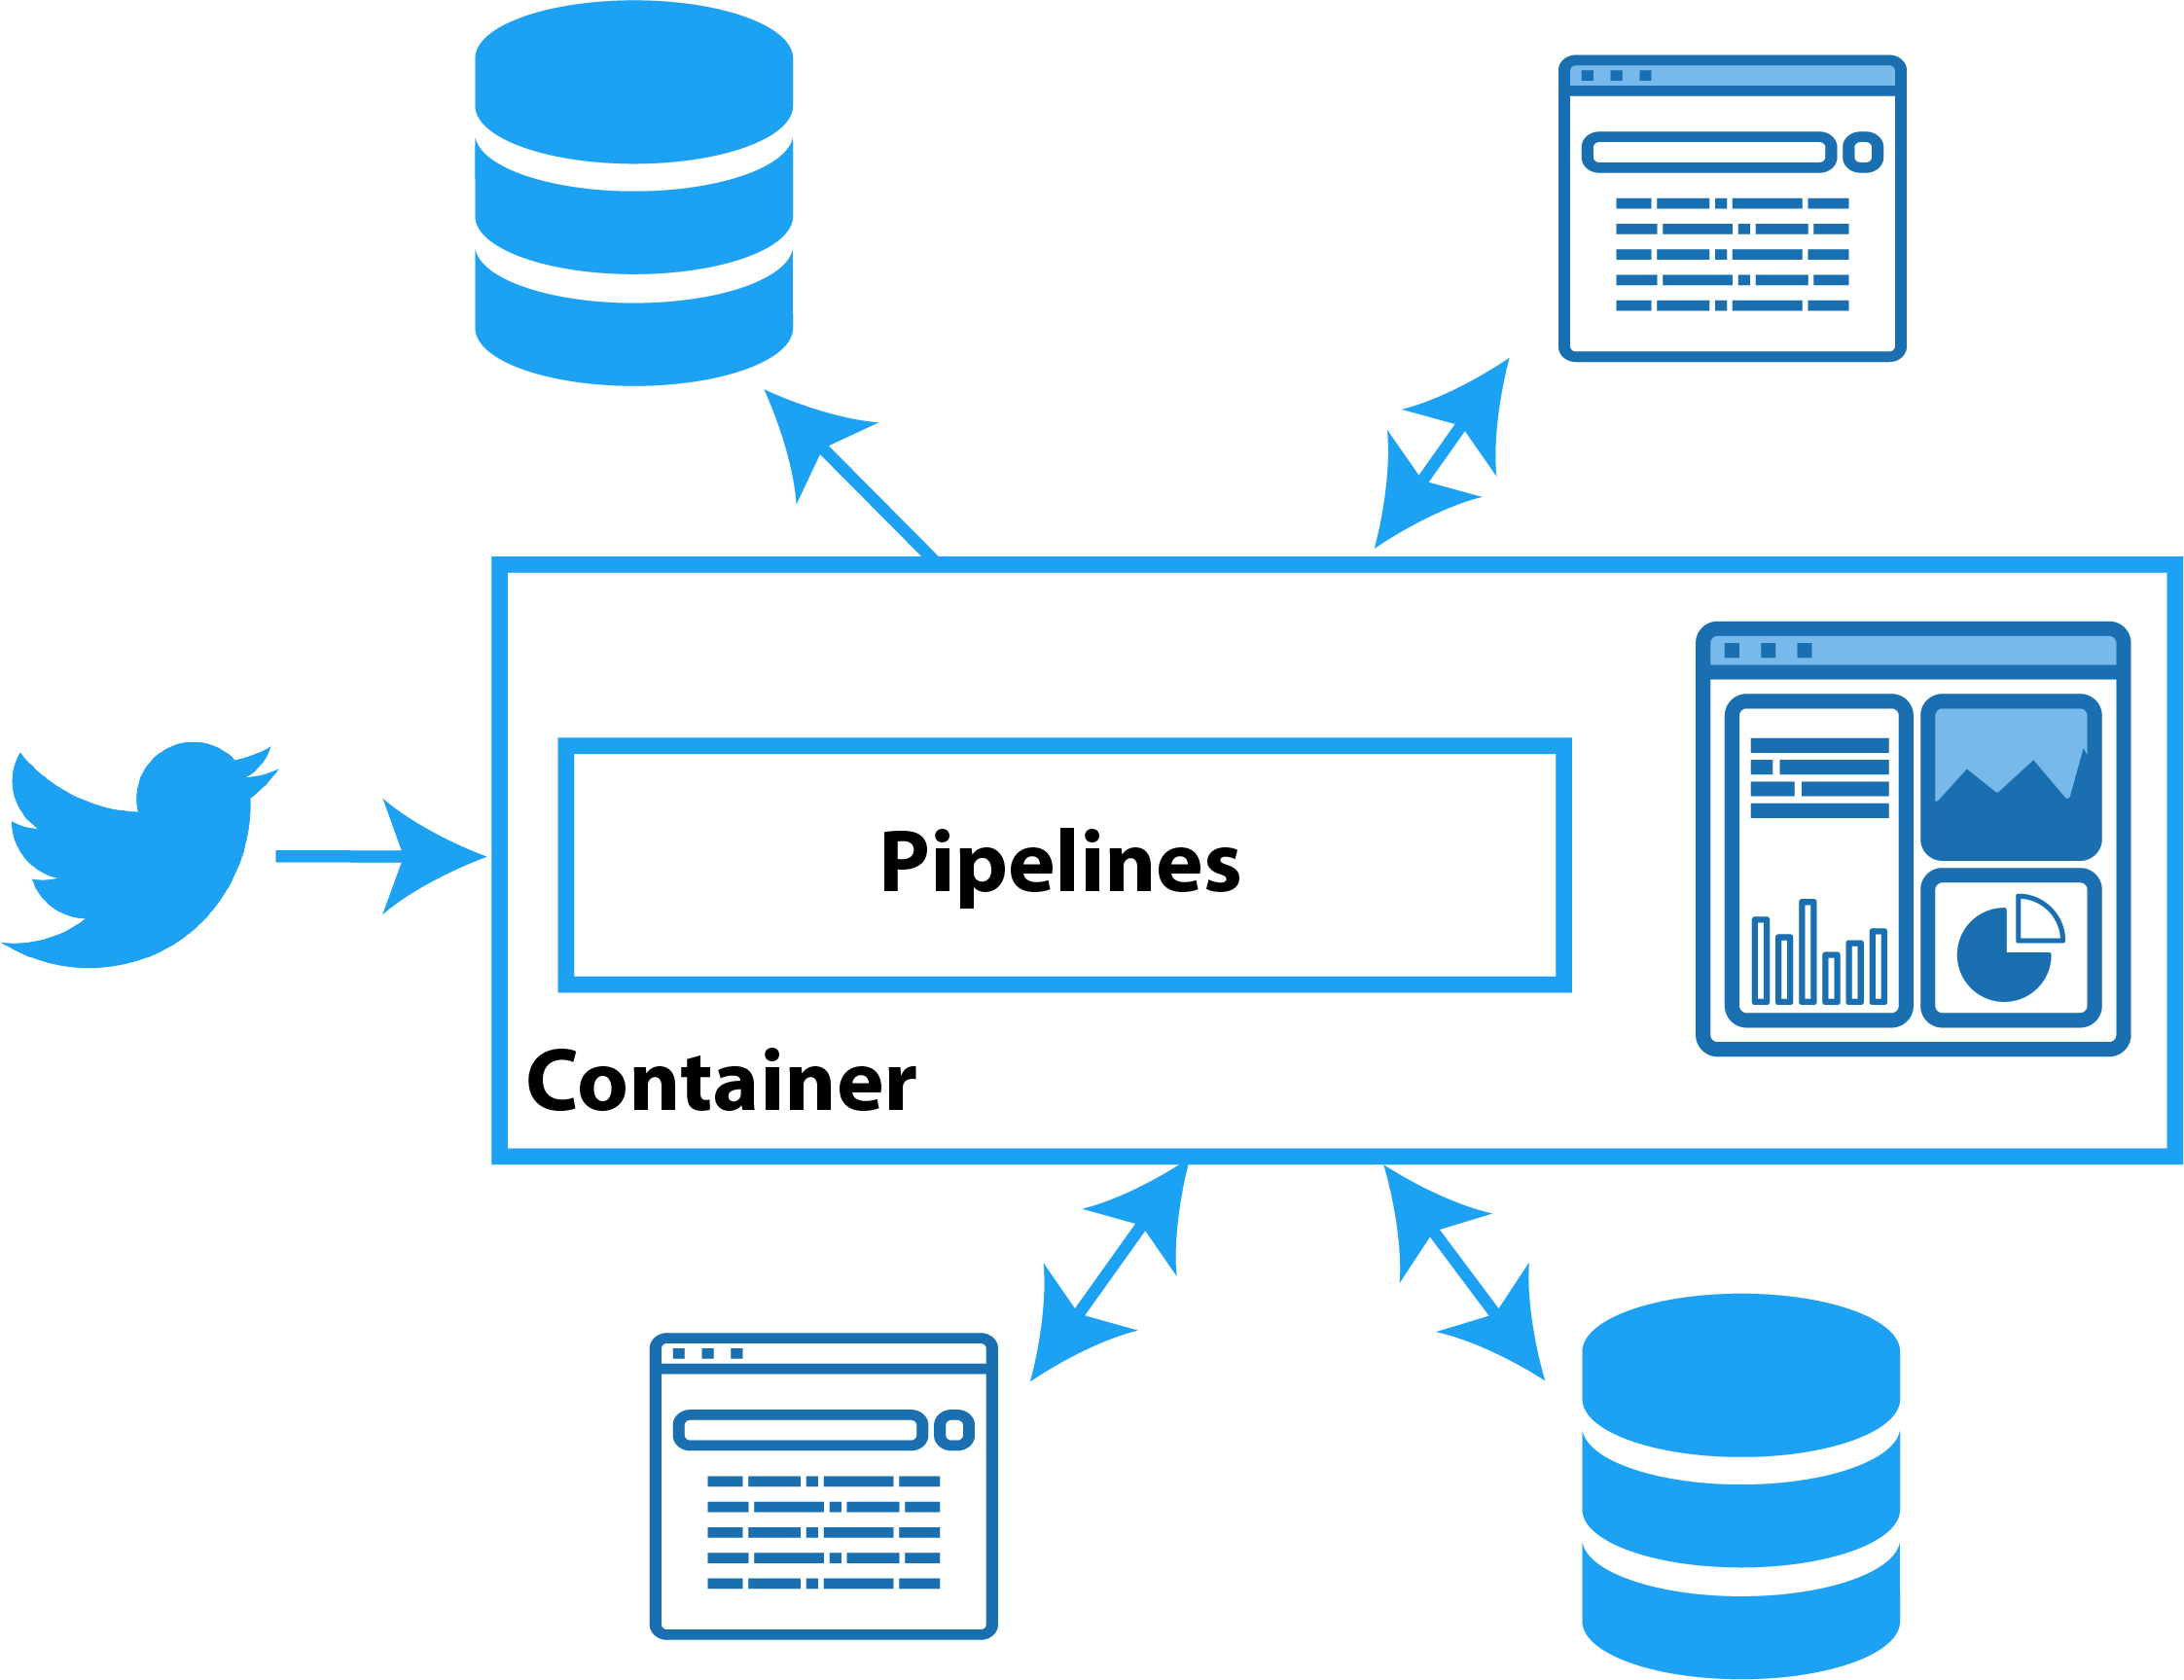
\includegraphics[scale=0.4 ]{images/architecktur_high_level_ohne.png}
	\caption{High Level L{\"o}sungsarchitekur}
	\label{fig:high_level_architecure}
\end{figure}
